\section{Введение}
\label{sec:Intro} \index{Chapter1}

В последние годы большие языковые модели (LLM) достигли значительного прогресса. Такие архитектуры уже сейчас способны эффективно решать широкий круг задач. В число таких задач входят: перевод, обработка и суммаризация текстовых данных, автоматизация бизнес-процессов через использование чат-ботов, а также многое другое. Однако действительно высоких результатов удается достигать только на моделях, в которых количество параметров исчисляется десятками и сотнями миллиардов. В то же время их разработка и поддержка требуют огромных вычислительных ресурсов, а среди качественных проблем главными остаются фактологические ошибки моделей и их неспособность адаптироваться к динамически изменяющимся данным.

При создании систем, способных поддерживать актуальность знаний в определенной предметной области, на сегодняшний день чаще всего используют метод Retrieval Augmented Generation (RAG) \cite{RAG}. Для этого подхода требуется формирование и поддержание документационных индексов, содержащих всю необходимую информацию по целевому домену. Наиболее частым сценарием применения подобных систем является Question-Answering (QA), когда задачей модели является генерация ответа на запрос пользователя с учетом документационной базы. Для этого в контекст генерации интегрируются релевантные фрагменты, извлечённые на основе пользовательского вопроса. 

В классической постановке такую архитектуру можно разделить на 4 ключевых блока:

\begin{enumerate}

  \item \textbf{\textit{Система предобработки данных.}}
  
    Компонент, который отвечает за обработку и разбиение исходных документов на более мелкие фрагменты (чанки). На этом этапе дополнительно может быть произведена очистка или обогащение метаданными (например, указание источника или номера главы).
    
  \item \textbf{\textit{Retriever.}}
  
    Часть системы, выполняющая задачу поиска релевантных фрагментов документации на основе пользовательского запроса. Может быть реализована с помощью классических статистических подходов, таких TF-IDF или BM25. На практике чаще всего представляют собой нейросетевую модель, отображающую текстовые фрагменты в векторное пространство высокой размерности для последующего поиска семантически близких фрагментов. 
    
  \item \textit{\textbf{Системы векторного хранения и поиска.}}
  
    Специализированное хранилище, оптимизированное для эффективного поиска по векторным представлениям. Оно индексирует чанки, преобразованные retriever’ом, и поддерживает операции поиска по метрике близости. Популярными решениями являются Qdrant (полноценная векторная база данных) и FAISS (библиотека для эффективного векторного поиска).

  \item \textit{\textbf{Генератор.}}
  
    Языковая модель, в контекст генерации которой подается запрос пользователя и извлеченные ранее текстовые фрагменты. Обогащение контекста документацией позволяет LLM генерировать ответ с учётом актуальной информации.
  
\end{enumerate}

Общая схема работы алгоритма изображена на рис. \ref{RAG pipeline intro}.

\begin{figure}[ht!]
    \centering
    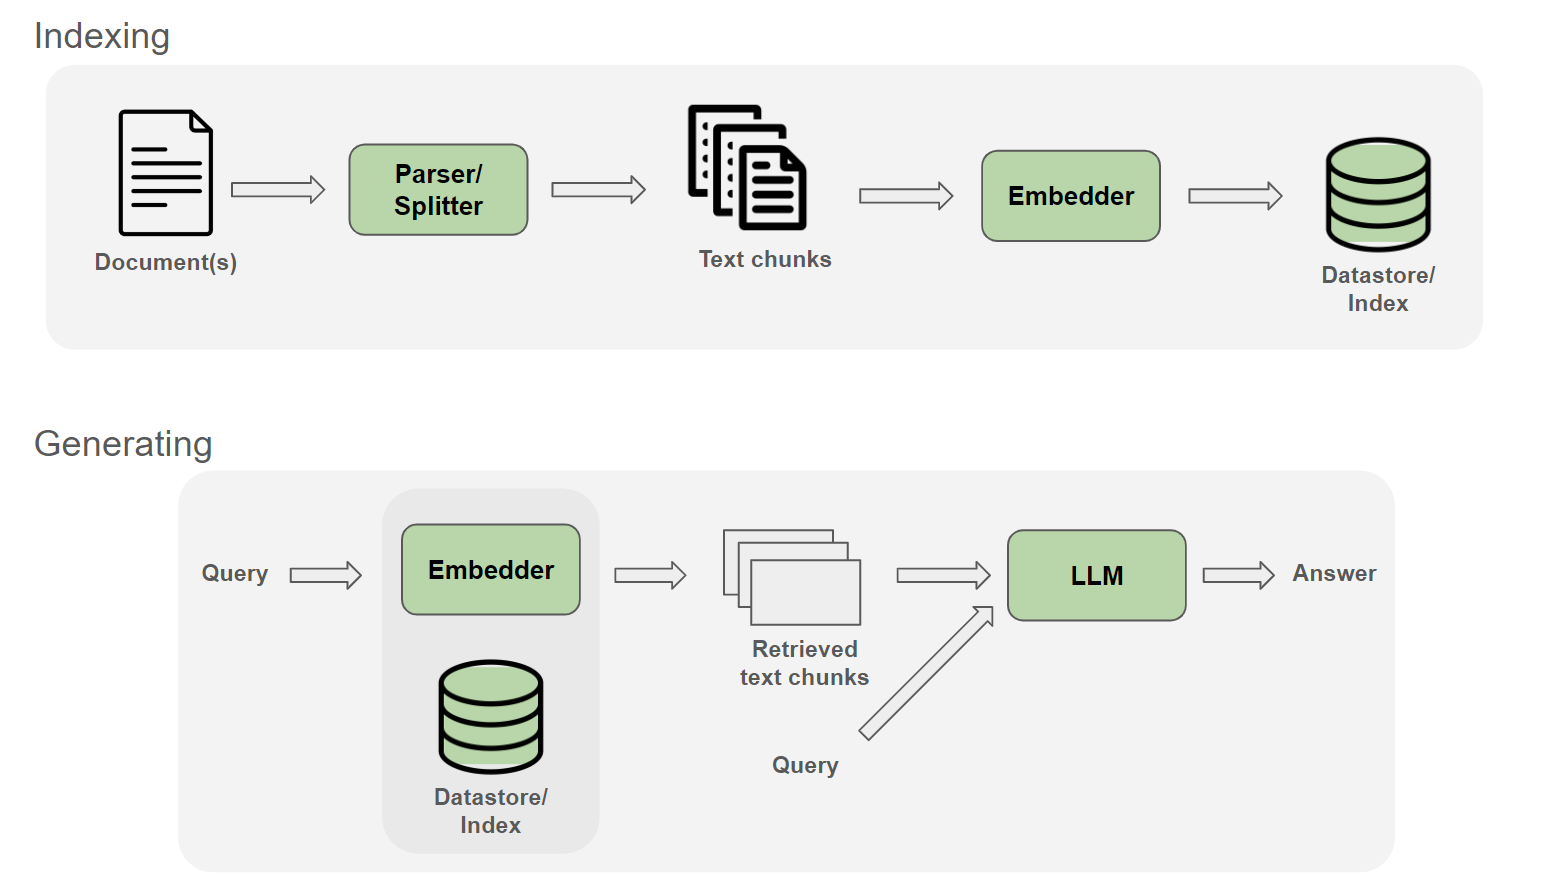
\includegraphics[scale=0.4]{images/rag_intro.png}
    \caption{Схема RAG pipeline.}
    \label{RAG pipeline intro}
\end{figure}

\newpage

% Этот подход крайне популярен и имеет множество вариаций. Так, например, алгоритм Graph RAG \cite{Graph_RAG} дополняет базовый принцип RAG за счёт извлечения сущностей и построения графа отношений по всему корпусу. В результате при поиске релевантного контекста можно осуществлять поиск по иерархически структурированному графу знаний. 

% Еще одним распространненным подходом является добавление модели ранжирования. Ее задачи состоит в изменении порядка извлеченных документов(лучшие впереди) и убирании избыточных документов. Продолжение этой идеи можно найти в работе <<RAG-Fusion: a New Take on Retrieval-Augmented Generation>> \cite{}   

Работа фокусируется на использовании языковых моделей в качестве интеллектуальных ассистентов для работы с обширными массивами документации. Многие современные компании активно разрабатывают и внедряют подобные системы в свою инфраструктуру. 

Технология полезна как для внутренних сотрудников компаний благодаря оперативному доступу к релевантной информации, так и для улучшения взаимодействия внешних пользователей с продуктом. При формировании ответа ключевым фактором является его фактологичность и корректность.

Несмотря на подтверждённую эффективность и широкое распространение, архитектура RAG имеет ряд ограничений, связанных с качеством её генеративной компоненты. В научной литературе выделяются две ключевые проблемы:

\begin{enumerate}

  \item \textbf{\textit{Генерация ответов на основе ложного контекста.}}
  
    Согласно исследованию <<Large Language Models Can Be Easily Distracted by Irrelevant Context>> \cite{irrelevant_retrieve}, некорректный контекст в RAG может вызывать <<галлюцинации>> модели, основанные на ложной или нерелевантной информации. Возможны даже ситуации, когда LLM могла самостоятельно ответить на поставленный вопрос, однако при добавлении дополнительного контекста, ответ становился неверным (рис. \ref{Hallucinations}).

    \begin{figure}[h!]
        \centering
        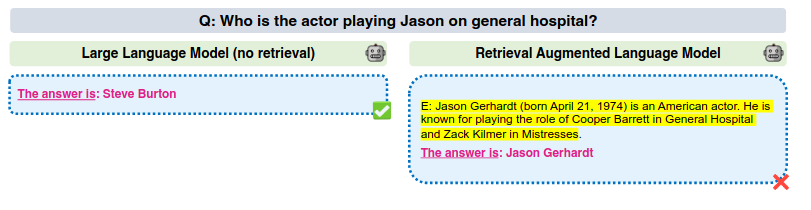
\includegraphics[scale=0.5]{images/hallucinations.png}
        \caption{Неверный ответ из-за нерелеватного контекста, взято из \cite{irrelevant_retrieve_ralm}}
        \label{Hallucinations}
    \end{figure}

  \item \textbf{\textit{Зависимость от позиции релевантной информации.}}

    При использовании RAG-систем для генерации ответов часто применяют модели, поддерживающие обработку расширенных контекстов. Данный подход позволяет потенциально передать больше релевантной информации. И хотя с технической точки зрения нет проблемы в реализации архитектур с большим или даже неограниченным контекстом, однако качество ответов моделей в таких сценариях значительно ухудшается. 

    Применительно к задаче извлечения информации эта проблема подробно описана в статье <<Lost in the Middle: How Language Models Use Long Contexts>> \cite{lost_in_the_middle}. Результаты исследования показывают, что LLM по умолчанию плохо справляются с извлечением информации из большого объёма разрозненных документов, фокусируясь преимущественно на информации в начале и в конце (рис. \ref{Lost in the middle}). Это приводит к снижению качества генерации, вплоть до уровня ниже, чем при отсутствии вспомогательных документов.

    \begin{figure}[h!]
        \centering
        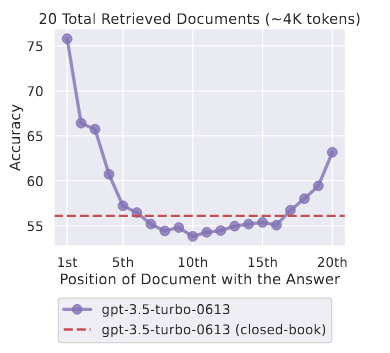
\includegraphics[scale=0.9]{images/Lost_in_the_middle.png}
        \caption{Качество ответа в зависимости от положения релевантной информации в контексте, взято из \cite{lost_in_the_middle}.}
        \label{Lost in the middle}
    \end{figure}
  
\end{enumerate}

Таким образом, возникает необходимость дообучения языковых моделей для повышения качества выделения информации из контекста. Для LLM критически важно не только извлекать полезные сведения из всего контекста генерации, но и иметь возможность находить и игнорировать шумовые или противоречивые фрагменты.

Важно отметить, что в рамках RAG-архитектур языковые модели выполняют функцию контекстуальных агрегаторов, синтезируя ответ на основе предварительно отобранной информации. На практике данную задачу, в отличие от классического QA, можно считать упрощенной, так как модель фокусируется не на генерации, а на структурировании ответа, что снижает требования к её «пониманию» изложенной информации.

Данная особенность открывает возможность оптимизации вычислительных ресурсов через применение компактных архитектур (объёмом 1-2 млрд параметров) при условии их специализированной адаптации под RAG-сценарии. Сохранение производительности в таких условиях достигается за счёт узкой специализации модели и усовершенствованных методов работы с контекстом.

Цель данного исследования — анализ, разработка и комбинация эффективных подходов дообучения LLM в сочетании с методами оценки качества генерации для задач RAG в условиях ограниченных вычислительных ресурсов.

\newpage
